\documentclass[letterpaper,12pt]{article}
\usepackage[utf8]{inputenc}
\usepackage[english]{babel}
\usepackage{graphicx}
\usepackage[printonlyused]{acronym}
\usepackage{tikz}
\usepackage{wrapfig}
\usepackage{lscape}
\usepackage{rotating}
\usepackage{epstopdf}
\definecolor{rfc}{RGB}{153,102,255}
\definecolor{land}{RGB}{88,74,72}
\definecolor{ada}{RGB}{46,111,211}
\definecolor{grad}{RGB}{22,101,105}
\definecolor{qda}{RGB}{179,179,179}
\definecolor{dtc}{RGB}{46,211,72}
\definecolor{voting}{RGB}{204,204,0}
\definecolor{bag}{RGB}{255,127,72}
\definecolor{mlp}{RGB}{255,66,66}
\definecolor{knn}{RGB}{51,102,0}
\definecolor{gau}{RGB}{153,51,51}
\usepackage[
    backend=biber,
    style=alphabetic,
    sorting=ynt
    ]{biblatex}
\addbibresource{references.bib}
\graphicspath{{./images/}}

\begin{document}
% Use the following at camera-ready time to suppress page numbers.
% Comment it out when you first submit the paper for review.
%\thispagestyle{empty}arg
    \title{Exloring Prediction of Global Bathymetry using pure Machine Learning}
    \author{Nicholas Moran}
    \date{01-05-20}
    \maketitle
    \section{Abstract}
\setlength{\parindent}{10ex}
This work attempts to demonstrate that ocean features can be used to train a \ac{ML} model for predicting bathymetry.
Ocean features were aggregated from a set of studies and placed into ~2 minute spatial grids representing earths oceans.
A set of regression models, classification models, and a novel classification model for this were analyzed in this work.
The training of these models were preformed using bathymetry data from the ETOPO2v2 dataset.
The performance of each model was evaluated using the bathymetry from this dataset, and subsequent metrics were produced and displayed in this work.
Results demonstrate that ocean features can be used to build a successful prediction model for bathymetry.
These results being the first reported in this work.

    
%Here is what I am about to tell you in this paper. Fairly informal and loose.
\section{Introduction}
\setlength{\parindent}{10ex}
The forefront in global bathymetry mappings are aggregations of predicted and measured sources. 
These \ac{EGM}s are the standard for measuring global bathymetry \cite{becker2009global}\cite{smith1994bathymetric}\cite{smith1997global}\cite{smith2010planning}.
While sonar platforms such as the Multi Beam Echo Sonar (MBES) \cite{farr1980multibeam} are the most accurate measurements of seafloor depth.
It is not cost and time effective to collect large swaths of \ac{MBES} bathymetry measurements.
\ac{EGM}s use satellite altimeter data to create gravitational models for predicting bathymetry at a fraction of the cost and time.
In general, these models predict bathymetry with a error of 190 meters \cite{jena2012prediction}.

\par
There has been much work using satellite altimeter derived gravity to predict bathymetry.
However, this work focuses on demonstrating the potential applications of \ac{ML} for predicting bathymetry.
The goal is to identify new potential approaches to predicting bathymetry.
I contribute to this domain by experimenting with regression and classification models fit to ocean feature data.
These experiments leading to a novel prototype model and a set of future experiments for predicting bathymetry.
    \section{Literature Review}
\setlength{\parindent}{10ex}
In this review I cover the different approaches for predicting bathymetry.
The two main methods for collecting bathymetry data are \ac{SDB} and \ac{EGM}.
There is also a third approach discussed that improves upon the idea of a \ac{EGM}.
I also discuss echo sounders for precise measurements of bathymetry \cite{farr1980multibeam}.

\subsection{Machine Learning}
Machine Learning can be defined as the process of fitting a model to data with a algorithm \cite{bishop2006pattern}.
Predictions can then be produced from the models by supplying new data.
To validate the predictions, the supplied data's result is known.
For example, a model is trained to predict if a image contains a car.
Data from the images are extracted and used to train the model.
Images with cars can be considered positive images.
Images with out cars can be considered negative images.
New images that are labeled as positive or negative are given to the model for validation.
If the model successfully predicts the labels it will have a high accuracy and be a "valid" model.
The two main types of models in Machine Learning is classification and regression models.
There are several high level descriptions of classification and regression models including: supervised learning, unsupervised learning, and reinforcement learning.

\par
Classification models are models that predict a discrete value.
For example, the car model mentioned earlier.
The model predicts a discrete value of either positive or negative.
These types of models are effective at predicting values that can be grouped into "labeled" data.
Classification models can also be combined to form ensemble models.
A ensemble is a combination of "weaker" predictors to form a strong predictor.
%Include citations BELOW!!!!!
Examples of classification models used in this project include: Decision Trees, Naive Bayes, MLP Classifier, Quadratic Discriminant Analysis Classifier, and K Nearest Neighbors Classifier.
Examples of ensemble classifieres used in this project include: Random Forest Classifier, Ada boost, Gradient Boosting, Bagging, and Voting.

\par
Regression models predict a continous value.
For example, predicting water depth as a number is a continous value.
Where the range of predicted values is from sea level to the known depth of the ocean.
Essentially, this model represents a mathematical function where the input data is the function parameters.
This method is best when the desired result can not be grouped into discrete "labeled" data.

\par
Unsupervised learning describes a model that is trained without labels.
Meaning that the data does not have corresponding "ground-truth" values for predictions \cite{bishop2006pattern}.
Training a model without "ground-truth" is used for grouping similar values together programatically.
Ideal for identifying correlations in data that is otherwise unrelated and unlabeled.

\par
Supervised learning describes a model that is trained with labels \cite{bishop2006pattern}.
Training is guided or supervised by comparing results to labeled data.
This method of training is effective at fitting accurate models, and is used in this project for predicting bathymetry.
All models trained in this project use supervised learning.
Each model used will be discussed in subsequent sections.

\subsubsection{Bias and Variance}
%Describe the Bias and Variance relationship!
The generalized error of a model can be expressed in terms of bias and variance.
Bias is the average error of a model for different training sets.
Variance describes the sensitivity of the model to data.
These two terms are nessassary to understand the bias-variance problem.
This problem applies to all forms of supervised learning \cite{geman1992neural} and describes the indirect relationship of bias and variance.
The relationship being the minimization of bias often causing high variance, and minimizing variance often causing high bias.
Optimally, accuracte models should have a low bias and variance.

%Include image showing bias and variance here!!
\begin{figure}[]
    \centering
    \includegraphics{sphx_glr_plot_underfitting_overfitting_001.png}
    \caption{}
    \label{}
\end{figure}

\subsubsection{Decision Trees}
%Talk about decision trees here
Decision trees are supervised models that are used for classification or regression \cite{breiman2017classification}.
They are simple to understand and interpret due to their simple decision structure. 
They are suseptable to over fiiting and can create overly complex trees that do not generalize well.
Over fitting is where a model will fit to closely to a training set \cite{cawley2010over}. 
Making it unable to make accurate predictions on data outside of what was used in training.

\begin{figure}[]
    \centering
    \includegraphics{dtreesepal.png}
    \caption{}
    \label{}
\end{figure}

%Talk about random forest here
\par
The Random Forest Classifier is a ensemble of many decision trees \cite{breiman2001random}.
It fits a number of decision trees on various sub samples of the dataset.
This also helps to control over fitting because each tree is fit to a sub sample of the dataset.
It averages the prediction of each tree to make a more accurate prediction than any single tree.


\subsubsection{Boosting}
%Talk about Ada Boost here
Boosting describes a type of ensemble that is concerned with reducing bias.
The idea being to build base estimators sequentially and then use the results of each to train a different estimator with the intention of reducing bias.
Adaboost is an example of one such model \cite{freund1995desicion}.
Its core principle being the fitting of weak learners on many random samples of the training data.
This learners are then combined with a majority weighted vote. 
This process is iterated for the training phase.



%Talk about Gradient Boosting Here
%Need to finish this paragraph....
\par
The gradient boosting classifier is an ensemble of trees similar to a random forest classifier.
In gradient boosting, decision trees are used as "weak" learners.
They are gradually added to the model in order to reduce the error.
This "gradient decent" approach is effective at building a successful classifier.
These types of boosting algorithms tend to overfit the model.
This can be solved by enforcing tree constraints and random sampling of data.


\subsubsection{Averaging}
Averaging ensembles operate by aggregating the predictions of many models trained on random sub sets of the training data.
Introducing randomization into the training will often reduce the variance of the resulting ensemble.
Bagging is a example of a averaging ensemble and has several implementations.
The Bagging ensemble uses a single classifier and fits instances of it to random samples of the training data.
The predictions are then aggregated and averaged for a final prediction.

%Talk about voting here
The voting classifier works by using the predictions of a set of conceptually different predictors as votes.
The majority vote (hard voting) or averaged vote (soft voting) is selected as the prediction.
This classifier is good for combining equally performing models in order to balance out individual weaknesses.

\subsubsection{K Nearest Neighbors}
%Talk about KNN for classification
The K Nearest Neighbors algorithm is a non-parametric algorithm for classification and regression \cite{altman1992introduction}.
K Nearest Neighbors for classification stores the instances of the training data and associated labels.
Predictions are made by computing the distance of new instances to the training set.

\subsubsection{Multi Layer Perceptron}
%Talk about MLP Classifier here!!!
% Include MLP picture here I guess
The Multi Layer Perceptron is a model that fits a function iterativly through a process called back propogation.
The MLP classifier is a neural network model that is based on the structure of the human brain.
It consists of many layers beginning with an input layer.
The middle layers are called the "hidden layers" and are each assigned a weight.
Back propogation is used during training to adjust the weights in the hidden layers.
These adjustments are made to in order to reach a more accurate prediction.
There can be many hidden layers of differnt depths.
% Probably need to say more about the MLP Classifier...
% Maybe some graphics and other bull jive. Maybe a algorithm???

\begin{figure}[]
    \centering
    \includegraphics{multilayerperceptron_network.png}
    \caption{}
    \label{}
\end{figure}


\subsubsection{Naive Bayes}
%Talk about Naive Bayes classifier here!!
The naive bayes classifier is based on applying the naive bayes theroem \cite{zhang2004optimality}.
The naive assumption of Naive Bayes is the conditional independence between pairs of features given the label.
Bayes theorem states the following relationship given class y and feature vector x.

% Put bayes theorem right here!!! Math mode I guess...


\subsubsection{Regression Models}
%Talk about Regression models used here...
Regression models are utilized for predicting continous values.
Specifically, regession is for approximating a function given a set of inputs to yield a output.
Linear regression is the simplest type and is concerned with fitting a linear combination of all training features.

% Put linear regression equation right here for the world to see YO

This project utilizes three regression models from sci kit.
The naive bayes\cite{sklearn_api}, logitic regression\cite{sklearn_api}, and svm regression\cite{sklearn_api} models are utlized for regression.


\subsection{Echo Sounders (\ac{MBES})(\ac{SBES}) }
Echo sounders have been mounted on vessels for decades to accurately measure bathymetry.
The purpose of this is often for the ship to avoid running aground.
However, survey vessels have utilized \ac{MBES} systems to reliably create bathymetry charts \cite{farr1980multibeam}.
This can give a accurate measurement of bathymetry in all water depths.
This methods downside is the cost and time required to map global coverage.
A vessel must transport these sensors, and potentially take decades of expensive surveys to gain full global coverage.

%VERY VERY VERY IMPORTANT SECTION....2018 paper contains good content for my thesis!
\subsection{Satellite Derived Bathymetry (SDB)}
\ac{SDB} is a precise method of predicting coastal bathymetry. 
This method relies on the phenomena of light passing through a water column at a certain depth described by the Beer-Lambert law \cite{chybicki2018three}\cite{vinayaraj2016satellite}.
Sunlight passes through the water column and is reflected by the sediment at the bottom.
Satellites measure the attenuated light that is reflected from the bottom and uses the wavelength to estimate the depth of the column.
The technique accounts for atmospheric light absorption, water surface reflection, attenuation through and out of the column, and reflectance from the bottom sediment.
Clear waters are the best environment for this method which has the potential to predict bathymetry with a small RMSE \cite{chybicki2018three}.

\par
This method is important for its ability to predict swaths of bathymetry in shallow water.
Shallow waters where larger vessels can not sail, and large swaths of coastal waters are measured by \ac{SDB} in a cost and time effective processs.
For example, the marsh lands of Louisiana where water depth is only deep enough for flat bed vessels.
This method also has use in the scope of national defense for predicting or identifying changes in shallow water bathymetry.
These changes can be caused by sediments or man made objects. 

\par
The limitations of the \ac{SDB} method are based on water depth and clarity.
As depth increases light is unable to pass through the water column to the bottom.
The depth that light can penetrate is determined by the characteristics of the water.
Clear water will allow for much deeper depths to be predicted, where as murky, cluttered water limits the maximum depth.
Environmental characteristics such as sediment composition and weather affect the clarity of water \cite{vinayaraj2016satellite}.

\par
Current \ac{SDB} models can predict bathymetry with a \ac{RMSE} of less that 2.5 meters at a maximum depth of 50 meters.
Work performed by \cite{vinayaraj2016satellite} has improved the depth by using blue light sensing techniques.
Work performed by \cite{chybicki2018three} improved the accuracy by using advanced regression models when measuring the wavelengths.
\ac{SDB} models are ideal for coastal areas with a high water visibility.

\subsection{Aggregated Earth Gravitational Models (EGM)}
Work performed by Smith and Sandwell \cite{smith1994bathymetric}\cite{smith1997global} pioneered the use of Earth Gravitational Models (EGM).
They proposed that the relationship between seafloor topography and sea surface gravity is conveniently related \cite{smith1994bathymetric}.
Their work identified the wavelength bands at which this relation holds true.
They identified the areas that could be predicted with this relationship and used sparse ship soundings to fill in gaps of their predictions.
Areas with large seamounts found the correlation to be strongest, while areas of flat sediments found the correlation to be weakest.
They named this technique the "Inverse Nettleton Procedure" and used a simple linear regression model to exploit this correlation and improve existing aggregated datasets.

\begin{equation}
    b(x) = D(x) + s(x)g(x)
\end{equation}

\par
Smith and Sandwell aggregated their predicted values from their \ac{EGM} with ship based Multi Beam Echo Sounding sonar data.
The sonar data is sparse, but provides accurate readings of the ocean's bathymetry.
This aggregation yielded global coverage up to 81 degrees.
The aggregation yielded prediction accuracy within ~100 meters in coastal waters, and ~200 meters in the global ocean space.

%Discuss the STRM Global Dataset here in detail....
\par 
This work was later improved in \cite{becker2009global}.
The model was substantially improved by increasing the number of ship soundings and increasing the aggregation sources.
Ten external datasets were aggregated for the SRTM30 grid.
Agencies in these sources include \ac{NAVO}, \ac{GEBCO}, \ac{NOAA}, \ac{NGA}, and \ac{JAMSTEC}.
These datasets include high resolution coastal bathymetry from around the world and greatly increased the global accuracy.

%Spelling check big time bruh
\par
The limitations of aggregated \ac{EGM}s is based on correlation uncertainty and unknown ocean features.
Sediment density drives the correlation between sea surface gravity and bathymetry.
A dense geoid will generate greater sea surface gravity than a less dense geoid.
Flat sea floors with a less dense composition can appear lower than normal.
This is all controlled by the scaling factor described in \cite{smith1994bathymetric} and shown in equation 1. 
However, there is not a optimal scaling factor for the entire world.
Identifying an optimal scaling factor for an area will require knowledge of the sediment type in the global scale.


\subsection{Machine Learning Optimized \ac{EGM}}
The aggregated \ac{EGM} is a physics based model that wants the relationship between gravity and bathymetry to be directly correlated.
This correlation is often non-trivial to define due to environmental factors.
The nondeterministic behavior is compensated by the scaling factor mentioned in the previous section.
Attempts to optimize this scaling factor have been made, and \ac{ML} has shown much promise in this regard.

\par
The work preformed by \cite{jena2012prediction} used \ac{ML} to optimize their gravitational regression models.
Instead of identifying an optimal scaling factor deterministically, they used an \ac{ANN} to optimize the scaling factor.
This was done using precise \ac{MBES} data as truth data and satellite altimeter data.
This method was tested on a localized swatch of ocean in the Arabian Sea.

\par
This optimization improved upon the current physics models.
Their model could predict bathymetry within a \ac{RMSE} of ~129 meters for flat sea floor.
Geoids resulted in a \ac{RMSE} of ~179 meters.
Both of these results are globally similar with aggregated models, while boasting increased accuracy in their localized training area of the Arabian Sea.

%\subsection{Machine Learning Models}
    \section{Overview}
\setlength{\parindent}{10ex}


    \section{Data Methodology}
\setlength{\parindent}{10ex}
The following chapter describes the data used in this project and how it was used for training.
Bathymetry data was extracted from the \ac{ETOPO}2v2 and used as truth value to train against a set of ocean features.
These ocean features were selected from a large set of aggregated features.
The selection was driven by a genetic algorithm that was used for speed as opposed to accuracy.
The trained models are then used to make predictions for the spatial resolution that was used in training.

\subsection{Bathymetry Data}
Data derived from predicted \ac{EGM} datasets represent the actual value of bathymetry at that point.
For example, predicted bathymetry datasets have a geospatial coverage.
These coverages vary in size by the resolution of the imagery.
Higher resolution imagery will have smaller coverages, and lower resolution will have more extensive coverages.
The predicted values used in this project represent an average of bathymetry across coverage. 
These predicted datasets are used as the truth values for training, but it is important to note that they are, themselves, predicted values.
Using this data is not intended to build accurate predictors, but to show that an accurate predictor can be built.

\par
The \ac{ETOPO} dataset is used in this project for bathymetry data.
This dataset is an aggregation of sparse \ac{MBES} ship soundings and predicted bathymetry from an \ac{EGM}.
It is an updated version of the original ETOPO2 dataset and was chosen because of the two minute resolution it offers.
\ac{ETOPO} was aggregated by the \ac{NGDC} which is a department of \ac{NOAA}.

\par
Land topography is included in the \ac{ETOPO} dataset.
This proved to be problematic in creating accurate bathymetry predictions.
Therefore, a mask was created to remove the land topography in all training datasets.
This is applied to the data before training to ensure that land data is not used in training.

%There is a better was to describe why the features were binned like this
%I want to describe the value that was added by binning my data into classes!
\par
Classification requires discrete class labels to predict.
To accommodate this requirement, the \ac{ETOPO} dataset was binned into discrete classes.
This binning was performed on 150 meter intervals.
This partitioning scheme was chosen to compare to the results from a similar work~\cite{jena2012prediction}.

\subsection{Training Data}
All feature data was aggregated from ocean and earth studies.
This data was then normalized and formatted for this project.
This aggregation was performed to gather a large set of testing samples regardless of the data's relevance.
For example, crust age may not be obviously useful for predicting bathymetry, but if it is useful, then feature selection will identify it as such.
This approach is fundamentally different to building a physics model.
For example, the mass of a geoid causes a vertical gravity gradient which creates ocean swells that can be measured by satellite altimetry.
Larger geoids will naturally affect the bathymetry of the sea floor.
This relationship is obvious and correlated in a measurable way.
On the other hand, machine learning can potentially identify relations in the data that otherwise will be difficult for a human to identify and model.

All features and their origin datasets can be seen in Table 1. %Insert point to figure yadaydada
Absent data points were either interpolated, or filled with default values.

\par
Figure~\ref{fig:bathyxfish} shows a plot of estimated fish biomass and bathymetry.
It can be conjectured that this relationship is more correlation that causality.
For example, biomass increases are not caused by shallow depths.
The shallow depth has more available light which allows for vegetation and energy supplies for more species, which could explain the relationship shown in this figure.

\par
Figure~\ref{fig:bathyxdensity} shows a graph of crust density and bathymetry.
This relationship may be more of a causality than correlation.
Denser crust is caused by many different factors that are separate from bathymetry.
It is possible that deeper water columns and the resulting weight contributed, but it can not be used to describe the correlation of the variables.

\par
In general, the features used in this project were a collection of potential predictors.
Features such as estimated oxygen, nitrogen, and salinity make sense for being related to bathymetry.
Other features such as crust density may not naturally be explained.
The feature selection was used to identify the best performing features.
Future study in the relationship of these features and how they benefit predicting bathymetry will be necessary.

\begin{figure}[htp]
    \centering
    \includegraphics[width=\textwidth]{Bathymetry_X_SS_BIOMASS_FISH_LOG10_MGCM2_Wei2010x.png}
    \caption{Graph of Bathymetry and Estimated Fish BIOMASS. Bathymetry is measured in meters and Fish Biomass is measured }
    \label{fig:bathyxfish}
\end{figure}

\begin{figure}[htp]
    \centering
    \includegraphics[width=\textwidth]{Bathymetry_X_SS_DENSITY_KGM-3_SACD_Aquarius_MISSION_MEANx.png}
    \caption{Graph of Bathymetry and Estimated Crust Density.
    Bathymetry is measured in meters and Crust Density is measured is milligrams per squared centimeter.}
    \label{fig:bathyxdensity}
\end{figure}

%This section is for defining the data being used in the experiment
%It should define where the data came from and its format
%I can also explain any of the special stuff I am doing (Binning for example)
%

\begin{table}[htp]
    \centering
    \begin{tabular}{ |p{0.5\textwidth} p{0.5\textwidth}| }
        \hline
            \textbf{Feature} & \textbf{Origin Study} \\
            \hline
            Mantle Density & CRUST1~\cite{laske2013update} \\
            LAND One Hot & ETOPO~\cite{national1988etopo} \\
            Crust Thickness & CRUST1~\cite{laske2013update} \\
            Low, Mid, High Crust Density & CRUST1~\cite{laske2013update} \\
            Estimated Current East, North, Mag & HYCOM~\cite{chassignet2009us} \\
            Sea Nitrate, Phosphate, Salinity Measurements & NASA Studies~\cite{meissner2018salinity,parekh2005decoupling}  \\
            Sea Temperature, Silicate Measurements & NASA Studies \\
            Sediment Thickness & CRUST1~\cite{laske2013update} \\
            BioMass Features &~\cite{wei2010global} \\
            Geoid Features & EGM~\cite{pavlis2008earth} \\
            Wave height, period & WAVEWATCH~\cite{tolman20072007} \\
        \hline
    \end{tabular}
    \label{table:FEATURE_LIST}
    \caption{List of Ocean Features used in Models for this Project.}
\end{table}
%I am using this section to introduce the feature selection method that I preformed
%Maybe I can flesh this out more and talk about it in def??
%Maybe make a diagram for the flow of the GA?
\subsection{Feature Selection}
Feature selection was used to identify the most relevant features for classification.
This important step in the \ac{ML} pipeline removes noise from irrelevant data.
This work used a genetic algorithm approach for feature selection~\cite{yang1998feature}.
Other approaches that were considered included a grid search, dimensional analysis, and simple variable correlations.
These approaches were found to either take too long or simply not offer enough improvement to the model.
The genetic algorithm approach gave relatively quick model improvements with little effort.
See Figure~\ref{fig:GA} for an illustration of a generic genetic algorithm.

\par
Using a genetic algorithm for feature selection is a simple application of the original process.
The initialized population is a set of random binary strings.
Each string has a character length equal to the number of features in our feature space.
The binary characters represent whether a feature is active or inactive.
Essentially these strings represent a set of features to use in training a model.
The fitness of that string is represented by the resulting model's accuracy.
Selection is performed by choosing the most accurate models and their characteristics then passing those onto to the next generation.
A simple crossover mutation of the strings is used along with a modest 5\% mutation rate.
Upon termination, the resulting fittest string is used as the selected features.


\begin{figure}[htp]
    \centering
    \caption{State Diagram of Generic Genetic Algorithm.
    The algorithm begins at an initialization state where the population is created.
    It then assigns a fitness attribute to each member of the population.
    This is the Fitness Assignment State.
    Then in the Selection State a selection is performed where the highest ranking members are selected for crossover and mutation.
    These states are designed to replenish the population.
    These actions are performed in the Crossover and Mutation States respectively.
    Finally, a stopping criterion is evaluated.
    If the population meets this criterion the algorithm exits, else, it goes to the Fitness Assignment State and repeats the previous steps.}
    \label{fig:GA}
    \includegraphics[scale=0.5]{genetic_algorithm.png}
\end{figure}

\par
Feature selection was used to remove noise from the training data.
This down sizing happened at a global scale.
It is possible that this may affect localized predictions where a feature is a strong predictor.
This was not tested in this work, but is an interesting question.
Identifying locally optimum features could lead to better models.


%This decribes how the grid files are used and oragnized...
%They are essentially binary files...
\subsection{Data Representation}
Representing the topography of the Earth can be done using a grid. 
Naturally, mapping a large circular sphere to a flat grid is not a direct conversion.
Latitude and Longitude represent the grid lines for the earth.
The data in the grid is a representation of the average value across an area.
This grid representation allows for ease of reading both by computers and humans.

\par
The spatial resolution of a grid defines its coverage.
It can be described as the height and width of a grid.
This height and width is not spatially constant.
For example, a cell at the equator is larger and covers more physical area than a cell at the poles.
However, this is the preferred to represent the data in a consistent and structured manner.

\par
All data in this project has been organized into two minute bathymetry grids.
A two minute bathymetry grid has a spatial resolution of 0.034 degrees per cell, which is approximately 3 kilometers of spatial coverage.
The grids have a column length of 5400 and a row width of 10800.
This resolution was chosen for experiments to conserve memory and time.
Larger grids have a exponentially larger memory and computational footprint.
I used the \ac{ETOPO}2v2~\cite{national1988etopo} dataset as the source of the two minute bathymetry grid.
Finer resolution datasets exist, such as the SRMT30~\cite{becker2009global} at 30 second resolution, however, the two minute resolution offered a good balance of memory, accuracy, and computational costs.

\subsection{Metrics}
Metrics are useful for evaluating a model and determining its usefulness.
The metrics used in this paper were chosen with this goal in mind.
RMSE, R2, F1-score, and Balanced Accuracy are the metrics used in this paper.

RMSE stands for Root Mean Square Error. 

%\ref{fig:pairplot} Shows a pair plot of all the features used in training.
%The diagonal in the pair plot will show the correlation of point distributions in each individual plot.
%Each of the discussed plots were taken from data in the south Pacific ocean.
%This was done as a isolated demonstration of the data.
%Talk about the plots here and include them once seaborn has decided to stop being dumb...


%\begin{figure}[h]
%    \centering
%    \includegraphics[scale=0.5]{Bathymetry_X_SS_BIOMASS_MEGAFAUNA_LOG10_MGCM2_Wei2010x.png}
%    \caption{Graph of Bathymetry and Estimated MegaFauna Bio Mass}
%    \label{fig:bathyxfauna}
%\end{figure}





%\begin{figure}[h]
%    \centering
%    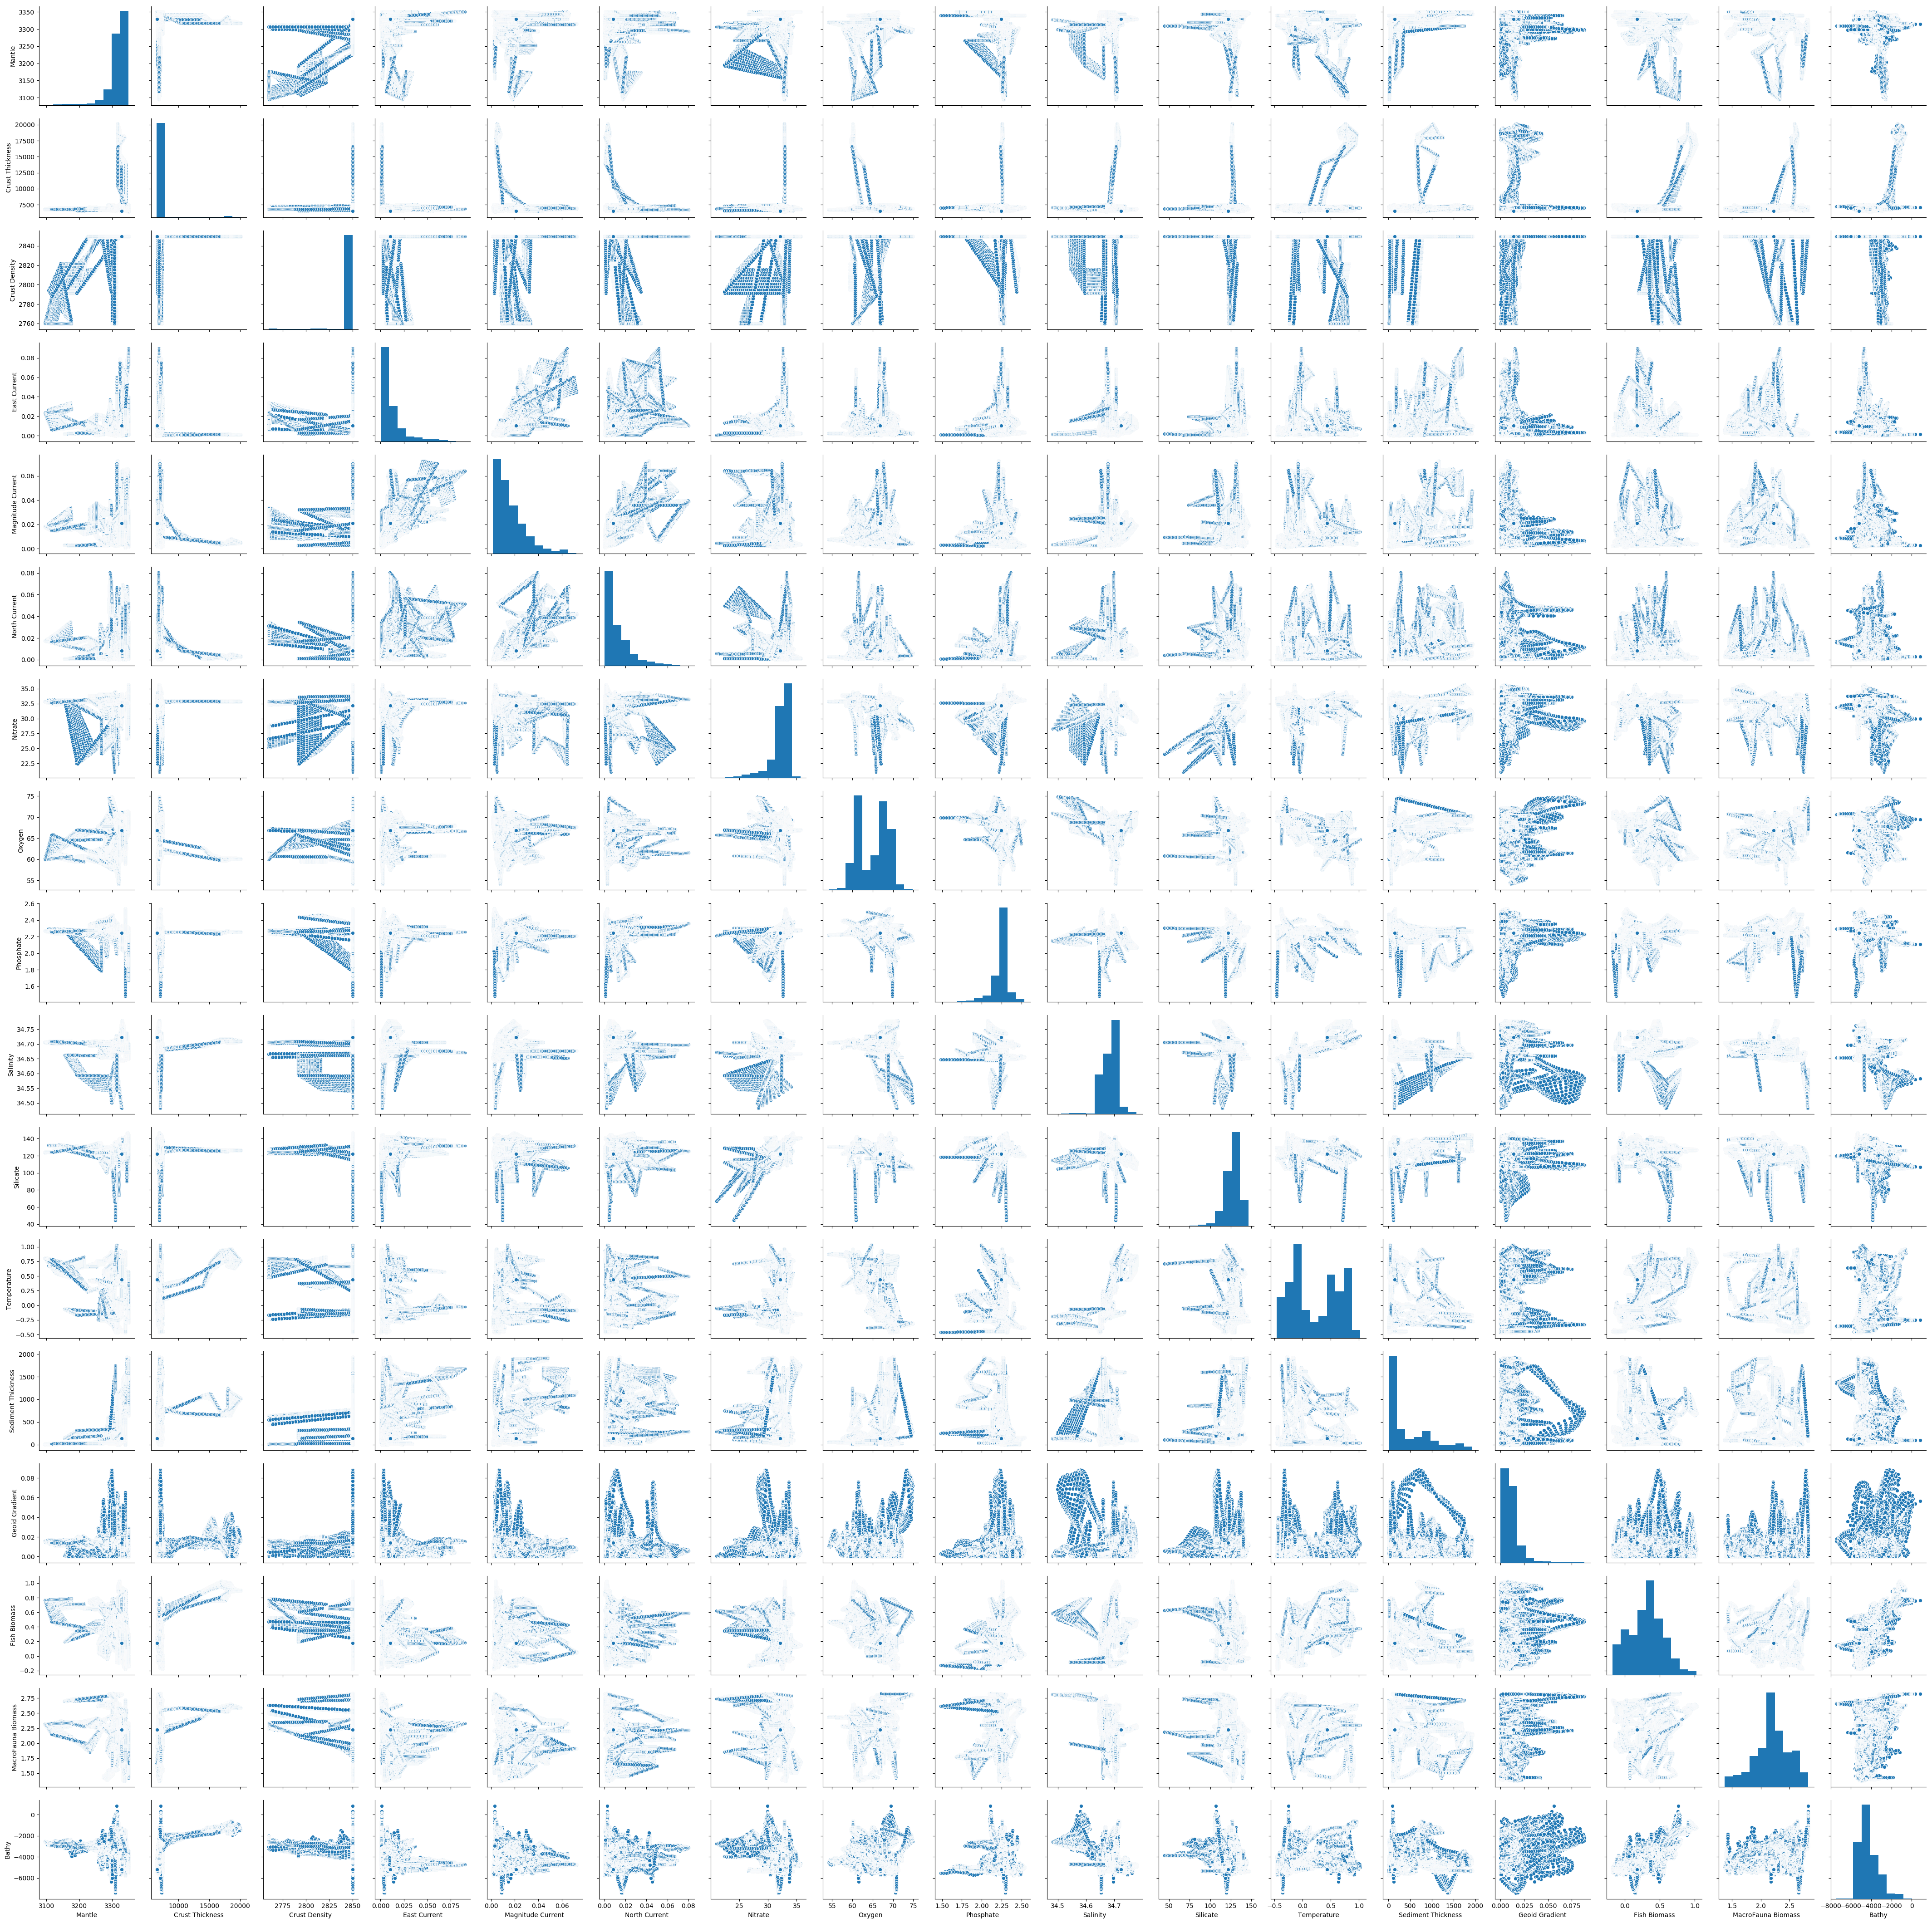
\includegraphics[scale=0.5]{pairplot.png}
%    \caption{Pair Plot of All Features Used in Training}
%    \label{fig:pairplot}
%\end{figure}

%Maybe I can talk about some of the correlations I preformed here???? A few graphs perhaps???
%Maybe talk about the PCC???
%Possibly need to talk about the breadth of features here....


    \section{Regression Results}
The first approach was to compare fitting a regression model against the feature space to a physics based \ac{EGM}.
Three models were fit to the data. 
A SVM regression model, a Naive Bayes regression model, and a simple linear regression model.

\begin{center}
    \begin{table}[htb]
        \begin{tabular}{|c c c|}
            \hline
				\textbf{Model} & \textbf{R Squared} & \textbf{RMSE} \\
				\hline
				SVM Regression & 0.841 & 365.23m \\
				Naive Bayes & 0.884 & 294.92m \\
				Linear Regression & 0.885 & 265.43m \\
				\hline
        \end{tabular}
        \label{table:REGRESSION_RESULTS}
        \caption{Regression Results}
    \end{table}
\end{center}

\subsection{Regression Results Discussion}
The regression preformed on the aggregated datasets under preformed compared to exsisting \ac{EGM}s.
\cite{jena2012prediction} achieved a \ac{RMSE} of ~175m in their optimised model.
The linear regression model I fit in this work is 90m less accurate than the optimised model used in \cite{jena2012prediction}.
However, the R squared score is high for each model. 
This shows that the data correlates well and that a good model can fit the data well.
While the regression results were uninspiring, the R2 score showed promise that a model can preform well.



%
%
%end{tabular}

% \begin{sidewaysfigure}[h]
%     \centering
%     \begin{tikzpicture}
%         \node[align=left,draw] 
% 		at ([yshift=-35pt]current bounding box.south)
% 		{%
% 			\begin{tabular}{c l c l c l c l}

% 				\begin{tikzpicture}
% 					\draw[fill opacity=0.5,fill=rfc] (0,0) rectangle (1,0.25);
% 				\end{tikzpicture}
% 				& RandonForestClassifier &  

% 				\begin{tikzpicture}
% 					\draw[fill opacity=0.5,fill=ada] (0,0) rectangle (1,0.25);
% 				\end{tikzpicture}
% 				& AdaBoostClassifier &

% 				\begin{tikzpicture}
% 					\draw[fill opacity=0.5,fill=grad] (0,0) rectangle (1,0.25);
% 				\end{tikzpicture}
%                 & GradientBoostingClassifier & 
% 				\begin{tikzpicture}
% 					\draw[fill opacity=0.5,fill=qda] (0,0) rectangle (1,0.25);
% 				\end{tikzpicture}
%                 & QDA \\ 
% 				\begin{tikzpicture}
% 					\draw[fill opacity=0.5,fill=dtc] (0,0) rectangle (1,0.25);
% 				\end{tikzpicture}
%                 & DecisionTree & 
% 				\begin{tikzpicture}
% 					\draw[fill opacity=0.5,fill=voting] (0,0) rectangle (1,0.25);
% 				\end{tikzpicture}
%                 & VotingClassifier & 

% 				\begin{tikzpicture}
% 					\draw[fill opacity=0.5,fill=bag] (0,0) rectangle (1,0.25);
% 				\end{tikzpicture}
%                 & Bagging &                
%                 \begin{tikzpicture}
% 					\draw[fill opacity=0.5,fill=mlp] (0,0) rectangle (1,0.25);
% 				\end{tikzpicture}
%                 & ANN \\
% 				\begin{tikzpicture}
% 					\draw[fill opacity=0.5,fill=knn] (0,0) rectangle (1,0.25);
% 				\end{tikzpicture}
%                 & KNN &

% 				\begin{tikzpicture}
% 					\draw[fill opacity=0.5,fill=gau] (0,0) rectangle (1,0.25);
% 				\end{tikzpicture}
%                 & NaiveBayes &
%                 \begin{tikzpicture}
% 					\draw[fill opacity=0.5,fill=land] (0,0) rectangle (1,0.25);
% 				\end{tikzpicture}
%                 & LAND \\
% 			\end{tabular}
% 		};
%     \end{tikzpicture}
%     \caption{}
%     \label{}
% \end{sidewaysfigure}
    \section{Optimized Grid Model}
\setlength{\parindent}{10ex}
%Purpose of this section is to identify the optimized grid structure.
%I need to check with Hoque to identify what I should and shouldnt include
%I need to consider rewording this and restructuring to manage the correctness for example etc.
Classification results showed that groups of classes had higher prediction rates in different models.
These results support that there is a optimum classifier for a area of the ocean.
The Grid Optimized Model Injector Classifier was created to test this theory.
This model is built upon the idea that there is not a optimal single model for predicting all of the worlds bathymetry.
It leverages several different models to predict bathymetry in a area by recording the best preforming models across a grid of the world.
This allows the model to use the optimal model for predicting bathymetry.

%Give the background for the idea in this section!
\subsection{Grid Optimizing Background}
According to the "No Free Lunch Theorem" \cite{wolpert1997no}, there is no optimal model to solve all problems.
For machine learning this theorem especially holds true.
To append onto the therm, there is not a single model that will optimally predict the entire globes bathymetry.
A model that preforms well in a area of the pacific may not preform well in the Atlantic.
Earth is a large planet with vastly different environments across degrees of latitude.
Likewise, the ocean ecosystem and topography changes relative to the location on the Earth.

\par
In the classification portion of this work there was evidence that a optimum model for a coverage exists.
This coverage should be designated to maximize accurate predictions.
Therefore, a proof of concept for this model will be to divide the Earth into coverages and test a set of models against each.
This will prove that a optimal set of coverages for a model does exist, and that localizing these models will yield benefit for predictions.

\begin{figure}[h]
    \centering
    \includegraphics[width=\textwidth]{optgriddraft.png}
    \caption{Graphic Showing the World Coverages and Successful Models}
    \label{fig:coveragegrid}
\end{figure}

\par
This proof of concept was implemented and executed against the existing discrete classed bathymetry data used in the classification section.
A Python script iterated across a grid of the world and trained the set of models.
Then compared the trained models and selected the best performing model.
Figure \ref{fig:coveragegrid} shows the results of this script.
Clearly, there are consistencies in depth, fault lines, and coast lines for the best models.
This supports the idea that dynamically injecting models will locally boost accuracy.

%In this section I am defining what the Grid optimization is and why it matters.
%There may be a better name for this?? Who knows really...
\subsection{Grid Optimizing}
This concept was further implemented by partitioning the world into coverages.
These coverages mirror the partitioned areas used in figure \ref{fig:coveragegrid} for simplicity.
For this project, I trained a set of classification models on each coverage to predict bathymetry.
The model that most accurately predicted bathymetry was then recorded and stored into a data structure.
This structure is a simple map of a bounding boxes and models.

%This is where I define what happens after the appropriate coverages have been found.
\par
The map structure is then used to create an ensemble that selects the optimal model for predicting in a coverage.
I call this ensemble the \textit{Grid Optimized Model Injector Classifier}.
Each model is retrained and validated using a 10 fold cross validation on the worlds set of data.
This trained model is then persisted and stored for use in predictions.
The model injector then references the optimized grid map and injects the best model for that coverage.
This reference is a simple geospatial query for the latitude and longitude of the bathymetry point.

\par
In theory, this injection will allow each model to perform to its optimum.
Each coverage highlights distinct characteristics that perform better for a certain estimator.
There are several patterns that can be gleaned from figure \ref{fig:coveragegrid}. 
Such as: consistencies with depth, along fault lines, and potentially sediment composition. 
% Reconsider this sentence....


\subsection{Results and Metrics}
%The world wide ETOPO bathymetry dataset \cite{national1988etopo} at two minute resolution is used for valadation and metrics.
%This dataset is treated as the ground truth for all predictions.
%During the experiment, a one third holdout was used for validation in some cases.
%For finding the optimum model for a coverage a 10 fold cross validation was utilized.

%Include metrics information here.... possibly graphs and a list of scores? I dont really know.

%I dont like how I worded this whole section...
%The idea here is that I want to say "Hey, these people did this research and found the their regression model preforms poorly for predicting seamounts espicially after 500m.
%I clearly noticed a similar trend, but saw better preformance from some models than others. 
%This research is to identify those coverages and then use those results to build a super classifier.
%These metrics are important for identifying where the models preform well. 
The Grid Optimized Model Injector improved the accuracy of predictions by ~5\%.
These gains are made by leveraging the "strongest" classifier for a coverage.
The balanced accuracy was generated using 10 fold cross validation on the worlds set of data.
The average F1 score across classes was generated by training against the trainsets in figure \ref{fig:trainset} and validated against the rest of the world.
These results are displayed in table \ref{table:GRID_OPT_RESULTS}.

\begin{table}[htb]
    \begin{tabular}{|c c c|}
        \hline
        \textbf{Model} & \textbf{Average F1 Score} & \textbf{Mean Balanced Accuracy} \\
		\hline
		Grid Optimized Model Injector & 0.83 & 0.862 \\
		\hline
        \end{tabular}
        \label{table:GRID_OPT_RESULTS}
        \caption{Regression Results}
    \end{table}
\end{center}

%Extending off the research preformed in \cite{jena2012prediction} these metrics allow the selection of the best preforming model.

%Maybe here I can have a table show casing the preformance of models or possibly statistics about the coverages??
%It will be intersting to see what has preformed better across the globe
%Also is intersting to see which models have preformed best overall.

    \section{Results}
\label{sec:results}
\setlength{\parindent}{10ex}

This section contains the results for each model observed by this work, including results for the regression, classification, and novel grid optimized model.
Each section includes figures representing the metric scores.

\subsection{Regression Results}
The \(R^2\) score for each model can be found in Figure~\ref{fig:r2_barplot_regression}.
The RMSE of each model can be found in Figure~\ref{fig:rmse_barplot_regression}.



\begin{figure}[htp]
    \centering
    \includegraphics[width=\textwidth]{worldtraininglocal.png}
    \caption{Initial training sets for regression. Testing was performed against the rest of the world.}
    \label{fig:trainset}
\end{figure}

% \begin{table}[htp]
%     \centering
%     \begin{tabular}{|c c c|}
%         \hline
% 		\textbf{Model} & \textbf{\(R^2\)} & \textbf{RMSE} \\
% 		\hline
% 		SVM Regression & 0.841 & 365.23m \\
% 		Naive Bayes & 0.884 & 294.92m \\
%         Linear Regression & 0.885 & 265.43m \\
% 	    \hline
%     \end{tabular}
%     \label{table:REGRESSION_RESULTS}
%     \caption{Regression Results}
% \end{table}

\begin{figure}[htp]
    \centering
    \includegraphics[width=\textwidth]{rsquared_barplot_regression.png}
    \caption{\(R^2\) score for each model. Higher values represent better performing models.}
    \label{fig:r2_barplot_regression}
\end{figure}

\begin{figure}[htp]
    \centering
    \includegraphics[width=\textwidth]{rmse_bar_regression.png} 
    \caption{RMSE for each model. Lower values represent lower error for a model.}
    \label{fig:rmse_barplot_regression}
\end{figure}

% \subsubsection{Regression Results Discussion}
% \cite{jena2012prediction} achieved a \ac{RMSE} of \~{}175m in their optimized model.
% The linear regression model I fit is 100 meters less accurate than the optimized model used in \cite{jena2012prediction}.
% However, the purpose of the test is not to achieve accurate predictions, but to identify if \ac{ML} models can be viable.
% Therefore, the accuracy of these models is less important than identifying the viability of the models.
% The training data used is essentially predicted bathymetry, but shows that fitting a model to true bathymetry will yield a similar result.
% Analyizing the \(R^2\) score gives evidence of the viability of the model.
% This score suggests that there are underlying relationships in the model that can be used to train a successful model.

\subsection{Classification Results}
\setlength{\parindent}{10ex}
The F1 results for each model can be found in Figure~\ref{fig:f1_barplot_classification}.
The Balanced Accuracy for each model can be found in Figure~\ref{fig:balacc_barplot_classification}.

\par
The Decision Tree classifier performed significantly worse than the other models.
The 47\% balanced accuracy is not usable for predictions.
Potentially, parameter tuning and feature selection could improve this model.

% \begin{table}[htp]
%     \centering
%     \begin{tabular}{|c c c|}
%         \hline
% 		\textbf{Model} & \textbf{Average F1 Score} & \textbf{Mean Balanced Accuracy} \\
% 		\hline
% 		Random Forest & 0.81 & 0.82 \\
%         Bagging & 0.80 & 0.79 \\
%         Decision Tree & 0.44 & 0.47 \\
%         \hline
%     \end{tabular}
%     \label{table:CLASSIFICATION_RESULTS}
%     \caption{Classification Results}
% \end{table}

\begin{figure}[htp]
    \centering
    \includegraphics[width=\textwidth]{f1_bar_classification.png}
    \caption{F1 score for each classifier. Higher values represent better precision and recall. From this, we see the Decision Tree does not make useful predictions.}
    \label{fig:f1_barplot_classification}
\end{figure}

\begin{figure}[htp]
    \centering
    \includegraphics[width=\textwidth]{balacc_bar_classification.png}
    \caption{Balanced accuracy for each classifier. Higher values represent higher accuracy.}
    \label{fig:balacc_barplot_classification}
\end{figure}

\subsection{Grid-Optimization Results}
The Grid Optimized Classifier used the results from Figure~\ref{fig:coveragegrid} as a decision function to select an \textit{optimum} model.
Simply, the classifier checks the location of the prediction for its corresponding grid in Figure~\ref{fig:coveragegrid}.
The model that performed best in that coverage is then used for classification.
This optimum model selection improved the prediction accuracy of the model by several percent.
See Figure~\ref{fig:grid_opt_barplot} for the results of the model.



\newpage

\begin{figure}[htp]
    \centering
    \includegraphics[width=\textwidth]{optgriddraft.png}
    \caption{World Coverages and Successful Models.
    Each square represents a coverage.
    The shaded color represents the model that was most successful in that coverage.}
    \label{fig:coveragegrid}
\end{figure}


\newpage
\begin{figure}[htp]
    \centering
    \includegraphics[width=\textwidth]{best_fit_percentage.png}
    \caption{Percentage of coverages where a model was "best fit".}
    \label{fig:pie_best_fit}
\end{figure}

\par
Figure~\ref{fig:coveragegrid} illustrates the coverages where each model performed best.
Figure~\ref{fig:pie_best_fit} shows the percentage that each model was a best fit.
The random forest classifier was the best fit model for a large portion of the oceans.
On the other hand, the Bagging classifier consistently performed well along the coast lines.
The reasons why these classifiers may have performed so well in those areas will be discussed/explained in Section 6.

\newpage
\begin{figure}[htp]
    \centering
    \includegraphics[width=\textwidth]{grid_opt_results.png}
    \caption{Grid Optimized Model results. Higher values represent better performing models.}
    \label{fig:grid_opt_barplot}
\end{figure}
%In this section I am defining what the Grid optimization is and why it matters.
%There may be a better name for this?? Who knows really...


    \section{Conclusion}
\setlength{\parindent}{10ex}
This study has experimented with three different experiments for predicting bathymetry with \ac{ML}.
Each experiment has improved upon the previous based on observations and analysis of the problem space.
Demonstrating that using a dataset of ocean features for building a model can be successful.
Improving the accuracy of these models will rely on access to accurate and complete ocean feature datasets.
Potentially, there are features not yet identified that could help with predictions.
In the future, iterating on features, models, and selection will lead to highly performant models.

    \section{Acronyms}
    \begin{acronym}
    \acro{MBES}{Multi Beam Echo Sounder}
    \acro{EGM}{Earth Gravitational Model}
    \acro{SDB}{Sattelite Derived Bathymetry}
    \acro{NAVO}{Naval Oceanographic Command}
    \acro{GEBCO}{General Bathymetric Chart of the Oceans}
    \acro{JAMSTEC}{Japan Agency for MarineEarth Science and Technology}
    \acro{NOAA}{National Oceananic and Atmospheric Administration}
    \acro{NGA}{National Geospatial Agency}
    \acro{RMSE}{Root Mean Square Error}
    \acro{ASW}{Anti Submarine Warfare}
    \acro{MIW}{MIne Warfare}
    \acro{ML}{Machine Learning}
\end{acronym}
    \printbibliography
\end{document} 